\section{Bias-tailoring I: choosing a schedule}\label{sec:choosing-a-schedule}

In this section we discuss differences between the $X^1Z^1$ and $X^1Y^1Z^1$ codes and their impact on the teraquop volumes.
We begin by considering the simpler case of direct parity measurement noise -- the simplicity here allows us to look closely at specific error mechanisms in order to better understand the two codes -- before we move to the more realistic but messier case of auxiliary qubit circuit noise.

\subsection{Differences}\label{subsec:differences}

We first outline the major differences between the two codes, and the expected effects on the teraquop volumes.
Some of these effects are in conflict with one another -- we will see numerically in the rest of this section which features ultimately dominate performance.

\begin{difference}\label{dif:XYZ_XZ_meas_per_detector}
    Detectors in the $X^1 Y^1 Z^1$ code consist of 12 measurements, while detectors in the $X^1 Z^1$ code consist of 6 measurements (\Cref{subsec:detectors}, \Cref{fig:detectors_XYZ_and_CSS}).
\end{difference}

The intuition is that the fewer measurements involved in a detector, the better.
This is because the more measurements that are involved, the more likely the detector is to be violated,
and more violated detectors means more marked vertices in the decoding graph,
which makes the job of the decoder harder\footnote{A more accurate metric capturing this intuition is that of \textit{detector likelihood} \cite{hesner2024using}. This is the total probability of a set of errors occurring that violate a given detector. In the comparison between the $X^1 Y^1 Z^1$ and $X^1 Z^1$ codes, measurement errors are the only errors that contribute differently to the detector likelihood -- all data qubit errors affect the detector likelihood in the same way across the two codes.}.
For example, MWPM has average-case runtime that's
approximately linear in the number of violated detectors,
provided the probabilities of qubit and measurement errors occurring are not too high~\cite{higgott2025sparse}.
Indeed, this is the intuition as to why the Bacon-Shor code has no threshold~\cite{gidney2023baconthreshold}.
So this difference between the two codes would suggest the $X^1 Z^1$ code might generally perform better, and therefore have a better teraquop volume -- especially for measurement-biased noise.

\begin{difference}\label{dif:XYZ_XZ_timelike_distance}
    The $X^1 Y^1 Z^1$ code implemented for $h$ rounds has a timelike distance of $h/2$, while the $X^1 Z^1$ code implemented for $h$ rounds has a timelike distance of $h/4$ (\Cref{tab:xyz_css_summary}, \Cref{fig:repeated_measurements_timelike_distances}).
\end{difference}

In contrast to \Cref{dif:XYZ_XZ_meas_per_detector} above, this difference favours the $X^1 Y^1 Z^1$ code;
based on this alone, one would expect the $X^1 Y^1 Z^1$ code to perform better than the $X^1 Z^1$ code in stability experiments,
i.e.\ have a smaller teraquop height $\tilde{h}$.
In particular, since the weight-$h/4$ timelike logical errors in the $X^1 Z^1$ code consist entirely of measurement errors,
one would expect this to be particularly relevant for measurement-biased noise.

\begin{difference}\label{dif:XYZ_XZ_hyperedges}
    All measurement errors in the $X^1 Y^1 Z^1$ code correspond to hyperedges in the decoding graph, while no measurement errors in the $X^1 Z^1$ code correspond to hyperedges (\Cref{tab:xyz_css_summary}).
\end{difference}

Recall that hyperedges are decomposed into ordinary edges in order to use a matching decoder like MWPM,
at the cost of losing some information about the likelihood of these errors occurring (\Cref{subsec:decoding_graph}).
But belief matching recovers much of this information (\Cref{subsec:decoding}).
Therefore belief matching performs best on codes where many errors correspond to hyperedges.
Accordingly, this difference suggests the $X^1 Y^1 Z^1$ code may perform worse than the $X^1 Z^1$ code under MWPM,
but improve a lot under belief matching.

\begin{difference}\label{dif:XYZ_XZ_logicals_pauli_type}
    In the $X^1 Z^1$ code, $E$ logical errors that consist of Pauli errors can only consist of $Z$ or $Y$ errors, whereas $M$ logical errors consisting of Pauli errors can only consist of $X$ or $Y$ errors.
    In the $X^1 Y^1 Z^1$ code, both types of logical error can be formed from all types of Pauli errors.
\end{difference}

This would seem to suggest that the $X^1 Z^1$ code can be better tailored to $Z$-biased noise in memory experiments,
for the following reason.
Recall that we are considering our toric DCCCs to implement just one logical qubit, rather than two, for simplicity and for better comparison with the more widely implementable planar case (\Cref{subsec:boundaries}).
In the $X^1 Z^1$ code under a $Z$-biased noise model, spacelike $E$ logical errors become more likely to occur,
and spacelike $M$ errors become less likely to occur.
But we can in effect cancel this out by changing the code dimensions.
Since the likelihood of spacelike $E$ logical errors occurring depends exponentially on the number of columns $n_E$ of hexagons in the code, and only linearly on the number of rows $n_M$ and the number of measurement rounds $h$, we can reduce the chances of such errors occurring by increasing $n_E$.
Similarly, if we decrease $n_M$ we increase the chances of spacelike $E$ errors occurring.
Altogether one might think we should be able to define a rectangular code with $n_E > n_M$,
such that we save qubits overall while maintaining the same protection against spacelike logical errors.
In the $X^1 Y^1 Z^1$ code this is not possible, because the noise being biased towards Pauli $Z$ errors doesn't increase or decrease the probability of either type of spacelike logical error occurring.

\subsection{Direct parity measurement noise results}\label{subsec:unrepetaed-direct-parity-measurement-noise}

Now we look at our simulation results.
\Cref{fig:X1Y1Z1_X1Z1_comparison} shows $\tilde{n}_E, \tilde{n}_M, \tilde{h}_E, \tilde{h}_M$ and the teraquop volume of the $X^1Y^1Z^1$ and $X^1Z^1$ codes for unbiased, $Z$-biased, and measurement-biased direct parity measurement noise.
We highlight two key points, and examine their relationship to the differences from the last subsection.

\begin{keypoint}\label{key:XYZ_XZ_best_and_worst}
    In all three noise models, the $X^1 Y^1 Z^1$ code under belief matching has the smallest teraquop volume,
    while the $X^1 Y^1 Z^1$ code under MWPM has the largest teraquop volume.
\end{keypoint}

This is exactly what was predicted by \Cref{dif:XYZ_XZ_hyperedges} -- all measurement errors in the $X^1 Y^1 Z^1$ code correspond to hyperedges in the decoding graph, which makes performance under MWPM worse.
But belief matching turns this bug into a feature.
Moreover, the effect becomes more dramatic the more the noise model is biased towards measurement noise.

This both agrees and disagrees with the intuition mentioned after \Cref{dif:XYZ_XZ_meas_per_detector} -- that the detectors in the $X^1 Y^1 Z^1$ consisting of twice as many measurements as in the $X^1 Z^1$ code would make the former perform worse, especially under measurement-biased noise.
While this is true for MWPM, using belief matching suffices to counteract this effect.
Indeed, the high number of measurements per detector and the fact all measurement errors violate four detectors are two sides of the same coin -- the latter being exactly what makes belief matching perform so well.
Similarly, the better timelike distance in the $X^1 Y^1 Z^1$ code (\Cref{dif:XYZ_XZ_timelike_distance}) doesn't seem to play a role under MWPM, but is consistent with performance under belief matching.

\begin{figure}[tbp]
    \centering
    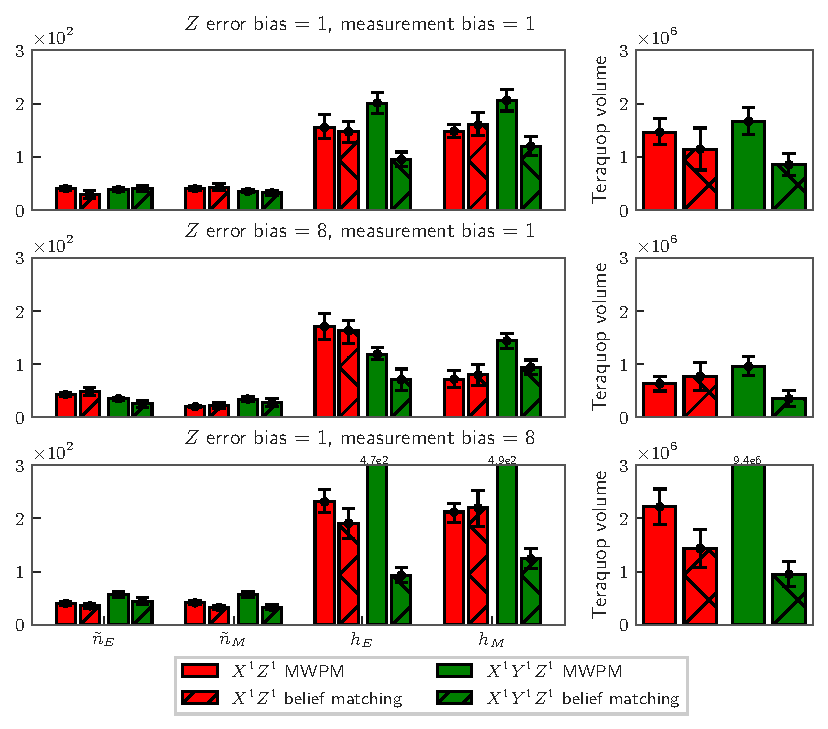
\includegraphics[width=0.9\linewidth]{figures/xyz_vs_css/X1Y1Z1_X1Z1_comparison.pdf}
    \caption{Comparison of $\tilde{n}_E, \tilde{n}_M, \tilde{h}_E, \tilde{h}_M,$ and teraquop volume of the $X^1Y^1Z^1$ and $X^1Z^1$ code decoded using MWPM and belief matching for unbiased, $Z$-biased, and measurement-biased phenomenological noise.
    In all cases, using belief matching rather than MWPM turns the $X^1 Y^1 Z^1$ code from the worst performer to the best performer (\Cref{key:XYZ_XZ_best_and_worst}).
    The difference in teraquop volumes comes primarily from the differences in teraquop height $\tilde{h} = (\tilde{h}_E + \tilde{h}_M)/2$ -- these dwarf the differences in teraquop footprints (\Cref{key:XYZ_XZ_footprints_similar}).
    This is thus an advert for analysing codes by looking at teraquop volumes rather than just teraquop footprints.}
    \label{fig:X1Y1Z1_X1Z1_comparison}
\end{figure}

\begingroup
\renewcommand*{\arraystretch}{1.5}
    \begin{table}[htbp]
        \centering
        \scalebox{0.9}{\begin{tabular}{|c|w{c}{1.8cm}|w{c}{1.8cm}|w{c}{1.8cm}|w{c}{1.8cm}|w{c}{1.8cm}|w{c}{1.8cm}|}
    %    \begin{tabular}{|c|c|c|c|c|c|c|}
            \hline
            & \multicolumn{3}{c|}{$X^1 Y^1 Z^1$} & \multicolumn{3}{c|}{$X^1 Z^1$} \\
            \cline{2-7}
            & \makecell{Direct parity\\ meas.} & \makecell{Meas.\\ noise} & Z noise & \makecell{Direct parity\\ meas.} & \makecell{Meas.\\ noise} & Z noise \\
            \cline{2-7}
            \hline
            \hline
            $d_{s, E}$ & $n_E$ & $n_E$ & $n_E$ & $n_E$ & $n_E$ & $n_E$ \\
            \hline
            $d_{s, M}$ & $\frac{4}{3}n_M$ & $\frac{4}{3}n_M$ & $\frac{4}{3}n_M$ & $\frac{4}{3}n_M$ & $\frac{4}{3}n_M$ & $\infty$ \\
            \hline
            $d_{t, E}$ & $h/2$ & $h/2$ & $h/2$ & $h/4 $ & $h/4 $ & $h/2$ \\
            \hline
            $d_{t, M}$ & $h/2$ & $h/2$ & $h/2$ & $h/4$ & $h/4$ & $\infty$ \\
            \hline
            $p_h$ & $5/9$ & $1$ & $1/3$ & $2/9$ & $0$ & $0$ \\
            \hline
        \end{tabular}}
        \caption{Differences in distances between the $X^1Y^1Z^1 $ and $X^1Z^1$ codes. The first four rows show graphlike distances of spacelike and timelike logical operators. The bottom row shows the \textit{hyperedge likelihood} -- the probability that a randomly chosen error in the noise model will correspond to a hyperedge in the decoding graph.
        Of note are that the $X^1 Z^1$ code has worse timelike distance when measurement errors are possible, but infinite spacelike and timelike $M$ distances when only $Z$ errors are possible.
        The $X^1 Y^1 Z^1$ code has a higher hyperedge likelihood in all cases, explaining why it performs the worst under MWPM but the best under belief matching (\Cref{key:XYZ_XZ_best_and_worst}).}
        \label{tab:xyz_css_summary}
    \end{table}
\endgroup

\begin{figure}[htbp]
    \centering
    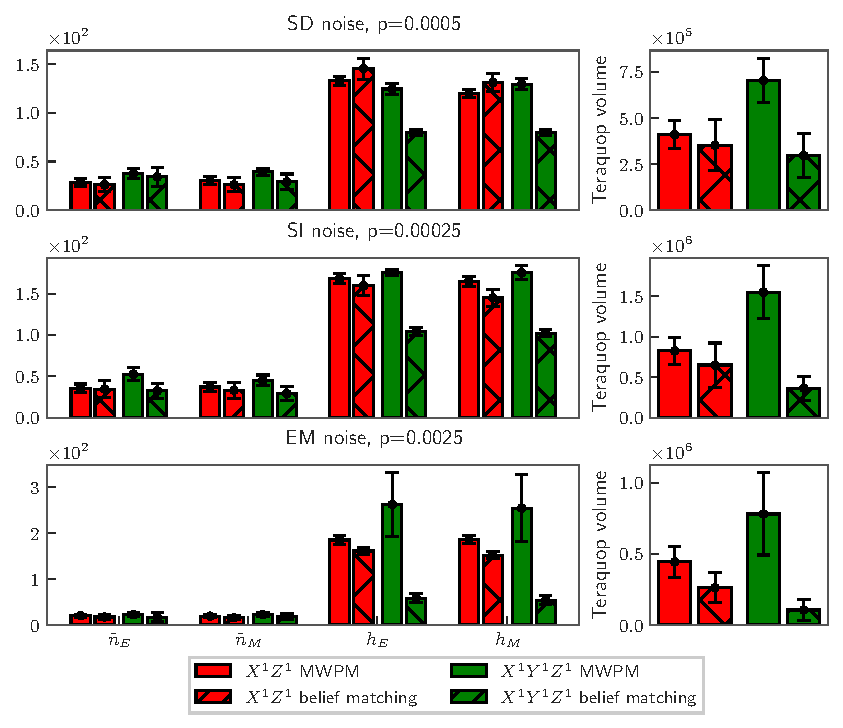
\includegraphics[width=0.9\linewidth]{figures/xyz_vs_css/X1Y1Z1_X1Z1_comparison_cln.pdf}
    \caption{Comparison of $\tilde{n}_E, \tilde{n}_M, \tilde{h}_E, \tilde{h}_M,$ and teraquop volume of the $X^1Y^1Z^1$ and $X^1Z^1$ code decoded using MWPM and belief matching for three circuit level noise models; standard depolarizing noise with $p=0.0005$, superconducting inspired noise with $p=0.00025$, and entangling measurement noise with $p=0.0025$.
    As in \Cref{fig:X1Y1Z1_X1Z1_comparison}, in all cases, using belief matching rather than MWPM turns the $X^1 Y^1 Z^1$ code from the worst performer to the best performer (\Cref{key:XYZ_XZ_best_and_worst}),
        and the most dramatic differences are to be found in the teraquop heights rather than footprints (\Cref{key:XYZ_XZ_footprints_similar}) -- especially for the entangling measurements noise model.}
    \label{fig:X1Y1Z1_X1Z1_comparison_cln}
\end{figure}

\begingroup
\renewcommand*{\arraystretch}{1.35}
\begin{table}[htbp]
    \centering
    \begin{tabular}{|c|w{c}{2.4cm}|w{c}{2.4cm}|w{c}{2.4cm}|w{c}{2.4cm}|}
%    \begin{tabular}{|c|c|c|c|c|}
        \hline
        & \multicolumn{2}{c|}{$X^1 Y^1 Z^1$} & \multicolumn{2}{c|}{$X^1 Z^1$} \\
        \cline{2-5}
        & SI \& SD noise & EM noise & SI \& SD noise & EM noise \\
        \hline
        \hline
        $d_{s, E}$ & $n_E$ & $n_E/2$ & $n_E$ & $n_E/2$ \\
        \hline
        $d_{s, M}$ & $\frac{4}{3}n_M$ & $\frac{2}{3}n_M$ & $\frac{4}{3}n_M$ & $\frac{2}{3}n_M$ \\
        \hline
        $d_{t, E}$ & $h/4$ & $h/2$ & $h/4$ & $h/4$ \\
        \hline
        $d_{t, M}$ & $h/4$ & $h/2$ & $h/4$ & $h/4$ \\
        \hline
    \end{tabular}
    \caption{
        Distances of the $X^1Y^1Z^1$ and $X^1Z^1$ codes.
        Note that the entangling measurements noise model halves the spacelike distances of both codes.
        Meanwhile the SI and SD noise models halve the timelike distances of the $X^1 Y^1 Z^1$ code,
        removing an advantage they had over the $X^1 Z^1$ code from \Cref{tab:xyz_css_summary}.
        These distances were obtained using Stim's function \texttt{shortest\_graphlike\_error}.
        For distance $4$ circuits we found the exact same distances when using the function \texttt{search\_for\_undetectable\_logical\_errors}.
        This second function takes errors that correspond to hyperedges into account.
    }
    \label{tab:xyz_css_summary_cln}
\end{table}
\endgroup

\begin{keypoint}\label{key:XYZ_XZ_footprints_similar}
    The differences in teraquop volume between the $X^1 Y^1 Z^1$ and the $X^1 Z^1$ codes are primarily due to differences in the number of rounds of measurements required to reach the teraqoup regime -- not in the number of physical qubits (footprint).
    
\end{keypoint}

That is, the differences in footprints $\tilde{n}_M \tilde{n}_E$ across codes and noise models are generally far smaller than the difference in the the teraquop heights $\tilde{h}$.
This contradicts the intuition from \Cref{dif:XYZ_XZ_logicals_pauli_type} -- we wondered whether the teraquop width $\tilde{n}_E$ and depth $\tilde{n}_M$ of the $X^1 Z^1$ code under $Z$-biased noise would be such that the footprint $f(\tilde{n}_E \tilde{n}_M)$ would be smaller than that of the $X^1 Y^1 Z^1$ code under this noise model.
Though $\tilde{n}_M$ is indeed smaller than that of the $X^1 Y^1 Z^1$ code, $\tilde{n}_E$ is larger.
That said, it could be that for a higher $Z$ noise bias than we simulated there could be a significant difference between $\tilde{n}_E \tilde{n}_M$ for the $X^1Z^1$ and $X^1Y^1Z^1$ codes.

A meta-point to make in light of \Cref{key:XYZ_XZ_footprints_similar} above is that using the teraquop volume rather than just the teraquop footprint was important.
Had we only used the teraquop footprint, we would not have seen the dramatic differences between the two codes and the two decoders, because these differences almost entirely show up in the teraquop heights rather than the footprints.
We claim this serves as evidence in favour of using teraquop volumes in future error correction simulations. 

In \Cref{tab:xyz_css_summary}, we summarise some important metrics.
We show the four types of distances of the two codes under the three different noise models,
and additionally show the \textit{hyperedge likelihood} $p_h$ -- the likelihood of an error in that noise model corresponding to a hyperedge in the decoding graph.


\subsection{Auxiliary qubit circuit noise results}\label{subsec:unrepeated-auxiliary-qubit-circuit-noise}

\Cref{fig:X1Y1Z1_X1Z1_comparison_cln} presents $\tilde{n}_E, \tilde{n}_M, \tilde{h}_E, \tilde{h}_M$, and the teraquop volume for the $X^1Y^1Z^1$ and $X^1Z^1$ codes under three auxiliary qubit circuit noise models.
Logical operator distances are summarized in \Cref{tab:xyz_css_summary}.
The results confirm the trends identified in \Cref{key:XYZ_XZ_best_and_worst}: the $X^1Z^1$ code performs best with MWPM, whereas the $X^1Y^1Z^1$ code is superior with belief matching.

Similarly, \Cref{key:XYZ_XZ_footprints_similar} holds, as differences in teraquop volume primarily stem from variations in the number of measurement rounds.
For SI and SD noise decoded with belief matching, $\tilde{h}_E$ and $\tilde{h}_M$ are reduced by a factor of two for the $X^1Y^1Z^1$ code.
Surprisingly, the timelike distance remains identical between the two codes, suggesting that distance alone is not always a reliable performance indicator.
A similar case was made in \Ccite{gidney2023pair}.

Despite simulating entangling measurement noise with a physical error rate ten times higher, the teraquop volumes remain of the same order of magnitude across all three auxiliary qubit circuit noise models.
